% Vortex Æther Model (VAM) — Full Manuscript
% Omar Iskandarani
\documentclass[12pt]{article}
\usepackage[utf8]{inputenc}
\usepackage{amsmath, amssymb, graphicx, geometry, hyperref, booktabs}
\geometry{margin=1in}
\title{Vortex Æther Model (VAM): Foundations, Formalism, and Physical Implications}
\author{Omar Iskandarani \\ Independent Researcher, Groningen, NL \\ \href{mailto:info@omariskandarani.com}{info@omariskandarani.com}}
\date{June 2025}

\begin{document}
    \maketitle

    \begin{abstract}
        This paper presents the Vortex Æther Model (VAM), a modern reformulation of the æther concept inspired by Einstein’s 1920 reinterpretation. VAM treats space as a structured, incompressible superfluid whose vorticity gives rise to mass, time, and gravity. Theoretical constructs are derived from hydrodynamic and topological first principles. We compare two symbolic mass models, derive time dilation expressions, and contrast VAM with historical and modern frameworks. A glossary and physical constants appendix support clarity and reproducibility.
    \end{abstract}

    \vspace{0.5cm}
    \textbf{Keywords:} æther theory, vortex dynamics, topological mass, helicity, Einstein, fluid models of spacetime

    \newpage
    \tableofcontents
    \newpage

    \section{Introduction}
    Einstein's evolving position on the æther concept—from rejection in 1905 to redefinition in 1920—opens the door to reinterpret the fabric of space not as void, but as a dynamic medium. The Vortex Æther Model (VAM) postulates that space is a non-viscous, incompressible superfluid whose topological vortex structures give rise to mass, time, gravity, and quantum-like behavior.

    \section{Historical and Philosophical Foundations}
    \subsection{Einstein's Æther Revisited}
    \begin{quote}
        \textit{“According to the general theory of relativity, space is endowed with physical qualities; in this sense, therefore, there exists an æther... space without æther is unthinkable.”} — Einstein, 1920
    \end{quote}
    We trace Einstein’s nuanced shift and compare it with VAM’s assertion that the æther behaves as a structured field with vorticity, swirl dynamics, and conserved circulation.

    \subsection{Kelvin and Maxwell on the Vortex Atom}
    Lord Kelvin's vortex atom theory and Maxwell’s ætheric mechanics both prefigure elements of VAM. Kelvin's topological critique—concerning the unbounded variety of knots—is addressed in VAM via circulation quantization, thermodynamic filtering, and reconnection thresholds.

    \section{VAM Theoretical Framework}
    \subsection{Core Postulates}
    \begin{itemize}
        \item Æther is an inviscid, incompressible superfluid.
        \item Vorticity \(\vec{\omega} = \nabla \times \vec{v}\) is a conserved quantity.
        \item Mass, time, and gravity emerge from vortex structures.
    \end{itemize}

    \subsection{Time Dilation from Swirl Clocks}
    \[
        \frac{d\tau}{dt} = \sqrt{1 - \frac{\omega^2 r^2}{C_e^2}}
    \]
    This relation parallels relativistic time dilation, with \(C_e\) acting as the maximum swirl speed.

    \subsection{Mass Formula from Vortex Geometry}
    \[
        M(p, q) = \frac{8 \pi \rho_{\ae} r_c^3}{C_e} \left( \sqrt{p^2 + q^2} + \gamma pq \right)
    \]
    Derived using vortex knot theory, helicity, and conservation principles.

    \section{Model Comparisons and Predictions}
    \subsection{Mass Models}
    \textbf{Model A (Preferred):}
    \[
        M(p, q) \propto \sqrt{p^2 + q^2 + \gamma pq}
    \]
    \textbf{Model B:}
    \[
        M(p, q) \propto p^2 + q^2 + \gamma pq
    \]
    Model A reproduces the electron, proton, and neutron masses within \textasciitilde0.1\% accuracy using \(\gamma \approx 0.0059\).

    \section{Constants and Glossary}
    \subsection{Selected Constants}
    \begin{tabular}{lllc}
        \toprule
        Symbol & Quantity & Value & Units \\
        \midrule
        $C_e$ & Vortex tangential velocity & $1.0938 \times 10^6$ & m/s \\
        $\rho_{\ae}$ & Æther vacuum density & $7.00 \times 10^{-7}$ & kg/m$^3$ \\
        $\gamma$ & Helicity-mass coupling & $\approx 0.0059$ & dimensionless \\
        $r_c$ & Vortex core radius & $1.4089 \times 10^{-15}$ & m \\
        \bottomrule
    \end{tabular}

    \subsection{Glossary of Key Terms}
    \textbf{Vorticity} \(\vec{\omega} = \nabla \times \vec{v}\): Local fluid rotation.

    \textbf{Helicity} \(H = \int \vec{v} \cdot \vec{\omega} \, dV\): Topological invariant quantifying twist and linkage.

    \textbf{Swirl Clock}: VAM clock influenced by local vorticity, analogous to gravitational time dilation.

    \textbf{Topological Charge}: Quantifies knot complexity and links helicity to mass.

    \section{Conclusion}
    VAM is not a throwback to outdated æther theories, but a coherent physical and mathematical realization of Einstein’s late æther. With topologically stable structures, experimentally testable predictions, and a closed-form mass model, VAM represents a modern, testable æther theory grounded in fluid dynamics.

    \section*{Figures}
    \begin{figure}[h!]
        \centering
        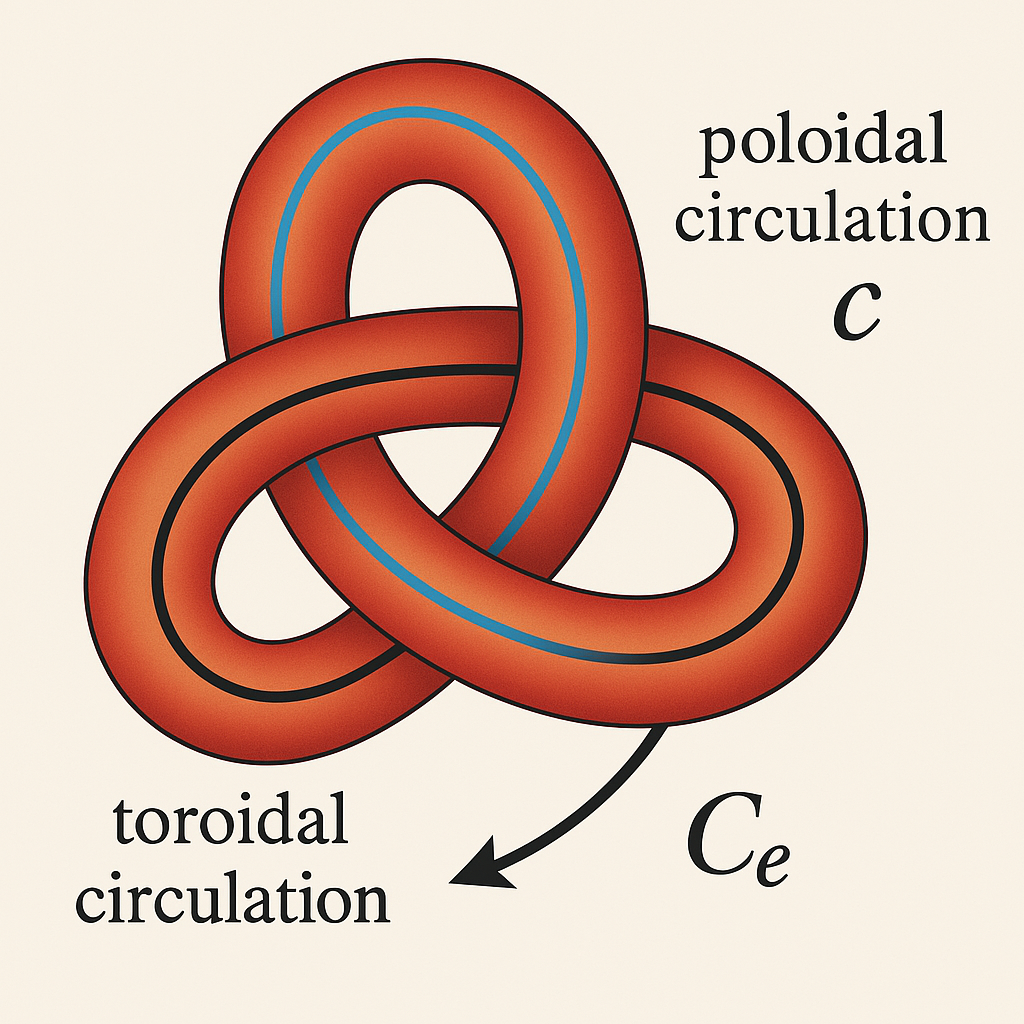
\includegraphics[width=0.6\textwidth]{../images/ChatGPT}
        \caption{Example of a torus knot $T(p,q)$ embedded in 3D space. Such knots model particles in VAM.}
    \end{figure}

    \section*{Appendices}
    \subsection*{A. Einstein on the Æther: Original Quotes and VAM Mappings}
    \textit{“Das Gravitationsfeld selbst kann als ein Zustand dieses Äthers angesehen werden.”} \rightarrow VAM: Gravity as pressure/vorticity coupling.

    \bibliographystyle{plain}
    \begin{thebibliography}{10}
        \bibitem{einstein1920} A. Einstein. Ether and the theory of relativity. University of Leiden, 1920.
        \bibitem{iskandarani2024} O. Iskandarani. Swirl clocks and vorticity-induced gravity. 2024.
        \bibitem{kelvin1904} Lord Kelvin. Baltimore Lectures on Molecular Dynamics, 1904.
        \bibitem{maxwell1875} J. C. Maxwell. Molecules. British Association Lecture, 1875.
    \end{thebibliography}

\end{document}
